
正如记录需求一样,也应该记录出现的架构。这当然不仅仅是为了拥有文档,它应该帮助每个参与项目的人提高生产力,使他们更好地理解自己的角色和最终产品需要什么。并不是所有的图表都对每个人都有用,但是可以试着从未来读者的角度来创建它们。

有许多框架可以记录愿景,其中许多框架服务于特定的领域、项目类型或体系结构范围。例如,如果对记录企业架构感兴趣,那么可能会对TOGAF感兴趣。这是\textit{开放组架构框架}的首字母缩写。它依赖于四个领域,即:

\begin{itemize}
\item 
业务架构(策略、组织、关键流程和治理)

\item 
数据架构(逻辑和物理数据管理)

\item 
应用架构(单系统的蓝图)

\item
技术架构(硬件、软件和网络基础设施)
\end{itemize}

如果将软件记录放在整个公司,甚至更广泛的范围内,那么这种分组就很重要。其他类似规模的框架包括由\textbf{英国国防部(MODAF)}和\textbf{美国等效机构(DoDAF)}开发的框架。

如果没有记录企业架构,若是刚刚开始架构自我开发道路,可能会对其他框架更感兴趣,例如4+1和C4模型。

\subsubsubsection{3.6.1\hspace{0.2cm}4+1模型}

The 4+1 view model was created by Philippe Kruchten in 1995. The author then claimed it is intended for "describing the architecture of software-intensive systems, based on the use of multiple, concurrent views." Its name comes from the views it consists of.

This model is widely known since it has been on the market for so long and does its job. It's well suited for bigger projects and while it can be used for small- and medium-sized ones as well, it can also turn out too complex for their needs (especially if they're written in an Agile way). If that's your case, you should try out the C4 model described in the next section.

A downside to the 4+1 model is that it uses a fixed set of views, while a pragmatic approach to document architecture would be to choose views based on the specifics of your project (more on that later).

A nice upside, on the other hand, is how the views link together, especially when it comes to scenarios. At the same time, each stakeholder can easily get the parts of the model relevant to them. This brings us to how the model appears: 

\begin{center}
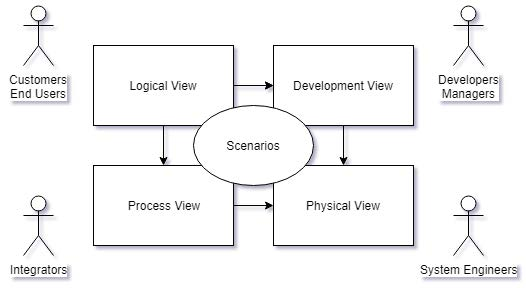
\includegraphics[width=0.8\textwidth]{content/1/chapter3/images/1.jpg}\\
Figure 3.1 – An overview of the 4+1 model
\end{center}

Actors in the preceding diagram are the ones most interested in their corresponding views. All the views can be represented using different kinds of \textbf{Unified Modeling Language (UML)} diagrams. Let's now discuss each view:

\begin{itemize}
\item 
\textbf{The logical view} shows how functionality is provided to users. It shows the system's components (objects) and how they interact with each other. Most commonly, it consists of class and state diagrams. If you have thousands of classes or just want to better show the interactions between them, you should also have communication or sequence diagrams, both being parts of our next view:

\begin{center}
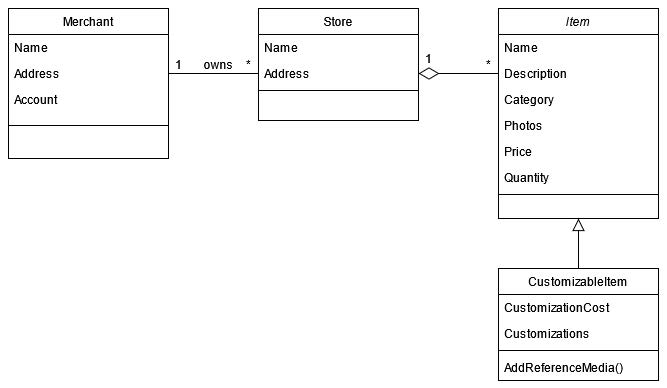
\includegraphics[width=0.8\textwidth]{content/1/chapter3/images/2.jpg}\\
Figure 3.2 – Class diagrams can be used to show what types we plan to have, along with their relations
\end{center}

\item 
\textbf{The process view} revolves around the system's runtime behavior. It shows processes, the communication between them, and interactions with external systems. It's represented by activity and interaction diagrams. This view addresses many NFRs, including concurrency, performance, availability, and scalability:

\begin{center}
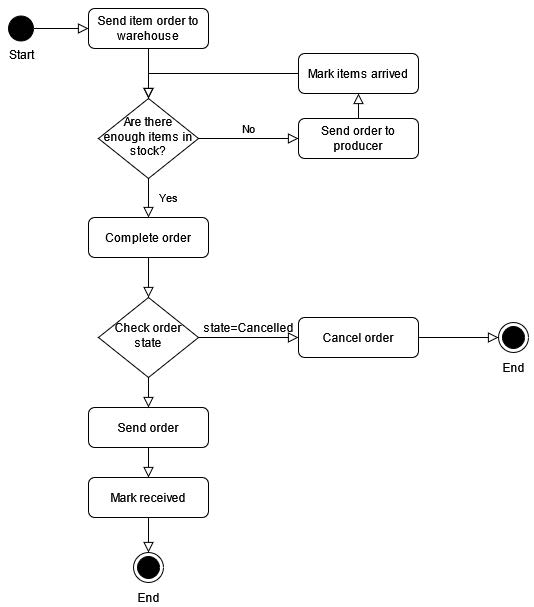
\includegraphics[width=0.9\textwidth]{content/1/chapter3/images/3.jpg}\\
Figure 3.3 – Activity diagrams are graphical representations of workflows and processes
\end{center}

\item 
\textbf{The development view} is for decomposing into subsystems and revolves around software organization. Reuse, tooling constraints, layering, modularization, packaging, execution environments – this view can represent them by showing a building-block decomposition of the system. It does so by using components and package diagrams:

\begin{center}
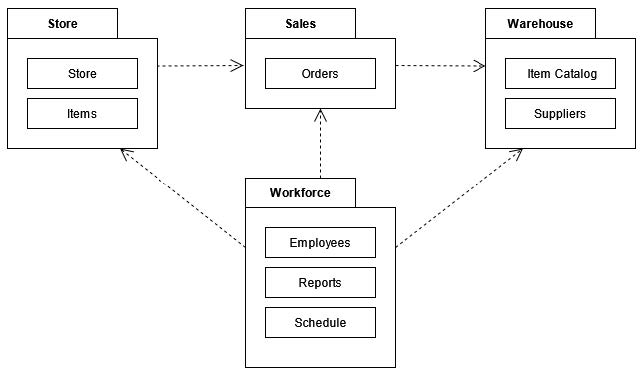
\includegraphics[width=0.8\textwidth]{content/1/chapter3/images/4.jpg}\\
Figure 3.4 – Package diagrams can show the parts of a system from a higher perspective, as well as dependencies or relations between specific components
\end{center}

\item
\textbf{The physical view} is used to map software to hardware using deployment diagrams. Aimed at system engineers, it can cover a subset of NFRs concerned with the hardware, for example, communication:

\begin{center}
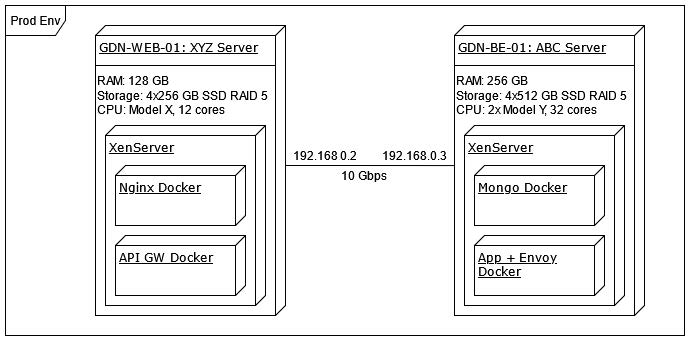
\includegraphics[width=0.9\textwidth]{content/1/chapter3/images/5.jpg}\\
Figure 3.5 – Deployment diagrams demonstrate the hardware on which each software component will run. It can also be used to pass on information regarding the network
\end{center}

\item
\textbf{The scenarios} are gluing all the other views together. Represented by use case diagrams, these can be useful for all stakeholders. This view shows whether the system does what it should and that it is consistent. When all other views are finished, the scenario view can be redundant. However, all the other views wouldn't be possible without usage scenarios. This view shows the system from a high level, while the other views go into the details:

\begin{center}
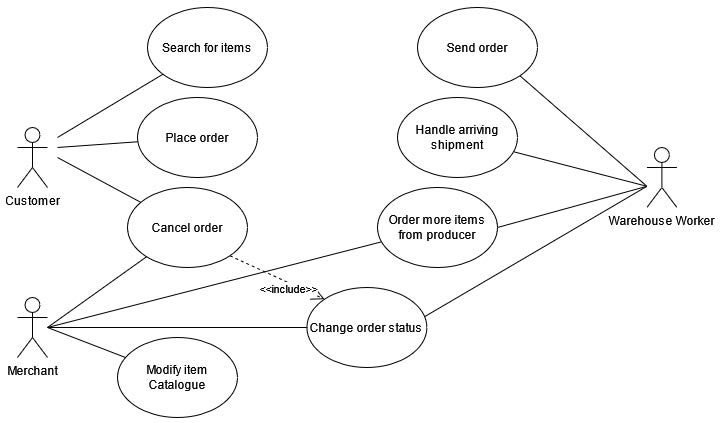
\includegraphics[width=0.9\textwidth]{content/1/chapter3/images/6.jpg}\\
Figure 3.6 – Use case diagrams show how specific actors interact with the system and how the interactions relate to each other
\end{center}

\end{itemize}

Each of those views is interconnected with the others and often they must coexist to show the full picture. Let's think about expressing concurrency. It can't be done using only the logical view, as it's more expressive to map them to tasks and processes; we need the process view. On the other hand, the processes will be mapped to physical, often distributed, nodes. This means we'll need to effectively document it in three views, each of which will be relevant for a specific group of stakeholders. Other connections between the views include the following:

\begin{itemize}
\item
Both logical and process views are used in analysis and design to conceptualize the product.

\item 
Development and deployment in conjunction describe how the software is packaged and when each package will get deployed.

\item
The logical and development views show how the functionality is reflected in the source code.

\item
The process and deployment views are meant to collectively describe NFRs.
\end{itemize}

Now that you're familiar with the 4+1 model, let's discuss another one, which is simple, yet extremely effective: the C4 model. We hope using it will be a blast (pun intended).

\subsubsubsection{3.6.2\hspace{0.2cm}C4模型}

The C4 model is a great fit for small- to medium-sized projects. It's easy to apply, as it's quite simple and it doesn't rely on any predefined notation. If you want to start diagramming using it, you can try out Tobias Shochguertel's c4-draw.io plugin (\url{https://github.com/tobiashochguertel/c4-draw.io}) for the free online drawing tool – draw.io (\url{https://www.draw.io/}).

In the C4 model, there are four main types of diagram, namely the following:


\begin{itemize}
\item
Context

\item 
Container

\item
Component

\item
Code
\end{itemize}

Just like zooming in and out using a map, you can use those four types to show more details of a particular code region or "zoom out" to show more about the interactions and surroundings of either a specific module or even the whole system.

The system context is a great starting point for looking at the architecture, as it shows the system as a whole, surrounded by its users and other systems that it interacts with. You can take a look at an example C4 context diagram here:

\begin{center}
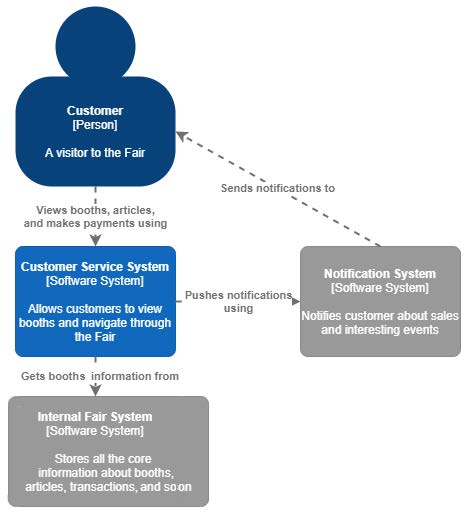
\includegraphics[width=0.9\textwidth]{content/1/chapter3/images/7.jpg}\\
Figure 3.7 – A C4 context diagram
\end{center}

As you can see, it shows the "big picture," so it shouldn't focus on specific technologies or protocols. Instead, think of it as a diagram that could also be shown to non-technical stakeholders. Just by looking at the diagram, it should be clear that there's one actor involved (the human-shaped depiction of the customer), who interacts with one of the components of our solution, namely, the customer service system. This system, on the other hand, interacts with two more, with each of the interactions described along with the arrows.

The context diagram we described is used to provide an overview of the system with few details. Let's now look at the other diagrams one by one:

\begin{itemize}
\item
\textbf{Container diagram}: This one is for showing the overview of the system internals. If your system uses a database, offers services, or just consists of certain applications, this diagram will show it. It can also show the major technology choices for the containers. Note that containers don't mean Docker containers; although each is a separately runnable and deployable unit, this diagram type is not about deployment scenarios. The container view is meant for technical people but isn't limited to the development team only. Architects, as well as operations and support, are the intended audience, too.

\item 
\textbf{Component diagram}: If you want more details about a specific container, this is where the component diagram comes into play. It shows how the components inside a selected container interact with each other, as well as with elements and actors outside the container. By looking at this diagram, you can learn about the responsibilities of each component and what technology it's being built with. The intended audience for component diagrams is mostly focused around a specific container and consists of the development team and the architect.

\item
\textbf{Code diagrams}: We finally come to code diagrams, which emerge when you zoom in to a specific component. This view consists mostly of UML diagrams, including class, entity-relationship, and others, and ideally should be created automatically from source code by standalone tools and IDEs. You should definitely not make such diagrams for each component in your system; instead, focus on making them for the most important ones in a way that allows them to actually tell the reader what you wanted to tell. This means that less can be more in such diagrams, so you should omit unnecessary elements from code diagrams. In many systems, especially smaller ones, this class of diagram is omitted. The target audience is the same as in the case of component diagrams.
\end{itemize}

You may find the C4 model lacking some specific views. If you're wondering how to demonstrate how your system should be deployed, for instance, you might be interested to learn that aside from the main diagrams, there are also a few supplementary ones. One of them is the deployment diagram, which you can see next. It shows how containers in your system are mapped to nodes in your infrastructure. In general, it's a simpler version of UML's deployment diagram:

\begin{center}
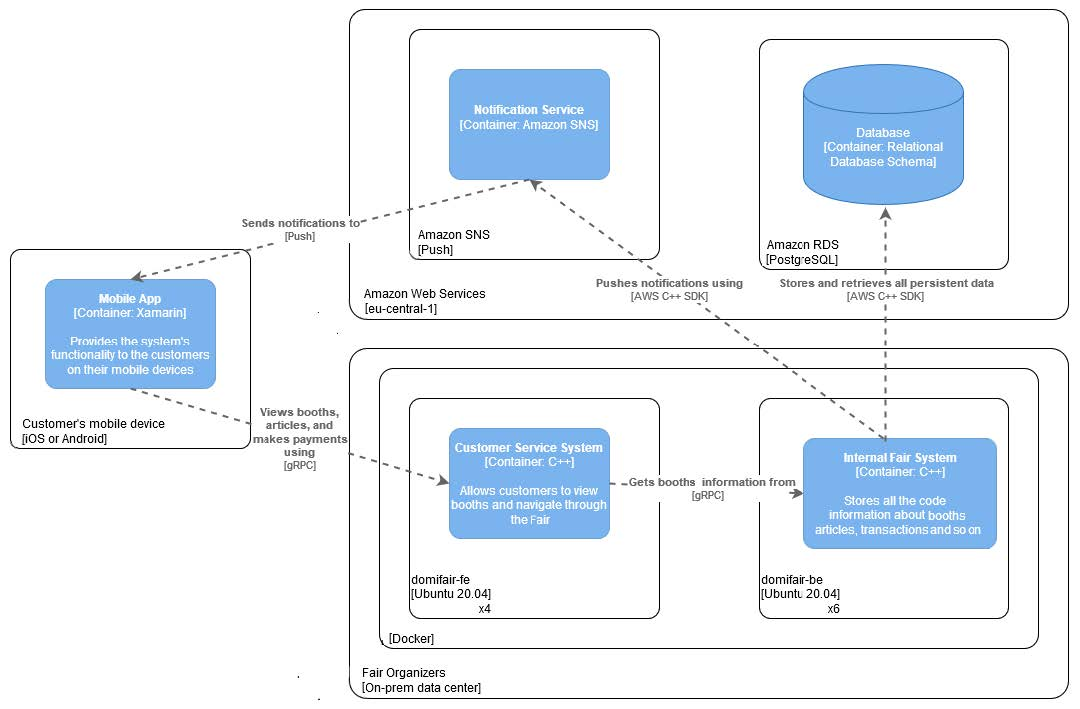
\includegraphics[width=0.9\textwidth]{content/1/chapter3/images/8.jpg}\\
Figure 3.8 – A C4 deployment diagram
\end{center}

Speaking of UML diagrams with regard to the C4 model, you might also wonder why it puts such little effort into presenting the system's use cases. If that's your case, then you should think about supplementing the preceding models with either the use case diagram from UML or perhaps think about introducing some sequence diagrams.

When documenting architecture, it's more important what you document and what knowledge you share than to follow a specific hard set of rules. Choose whatever tools suit your needs the best.

\subsubsubsection{3.6.3\hspace{0.2cm}记录敏捷项目中的架构}

In Agile environments, your approach to documenting architecture should be similar to the one about documenting requirements. First and foremost, consider who will be reading the materials you prepare to be sure you're describing the right things in the right way. Your documentation doesn't need to be a lengthy Word document. You can use presentations, wiki pages, single diagrams, or even recordings from meetings when someone describes the architecture.

What is important is to gather feedback on the documented architecture. Again, in the same way, as with the documented requirements, it's important to reiterate the documents with your stakeholders to know where to improve them. Even though this may seem like you're wasting time, if done properly, it should save you some time in terms of delivering the product. Good enough documentation should help newcomers to start being productive faster and guide more familiar stakeholders down the road. If you just discuss the architecture at some meetings, chances are, a quarter later, no one will remember why you made the decisions you made and whether they will remain valid in the ever-changing, Agile landscape.

Reiteration is important when creating documentation because most probably there will be some misunderstanding of an important detail or two. Other times, you or your stakeholders will gain more knowledge and decide to change things. Be prepared to go through the document at least a few times before it will be considered mature and done. Often, a few conversations over IM, phone, or in-person will help you finish it quicker and address any follow-ups that could arise, so prefer those to emails or other asynchronous ways of communication.


























